\documentclass[11pt,addpoints,answers]{exam}

%-----------------------------------------------------------------------------
% PACKAGES AND OTHER DOCUMENT CONFIGURATIONS
%-----------------------------------------------------------------------------

\usepackage[margin=1in]{geometry}
\usepackage{amsmath, amsfonts}
\usepackage{enumerate}
\usepackage{graphicx}
\usepackage{titling}
\usepackage{url}
\usepackage{xfrac}
\usepackage{natbib}
\usepackage{amssymb}
\usepackage{amsthm}
\usepackage{paralist}
\usepackage{epstopdf}
\usepackage{tabularx}
\usepackage{longtable}
\usepackage{multirow}
\usepackage{multicol}
\usepackage[colorlinks=true,urlcolor=blue]{hyperref}
\usepackage{algorithm}
\usepackage{algorithmicx}
\usepackage[noend]{algpseudocode}
\usepackage{float}
\usepackage{enumerate}
\usepackage{array}
\usepackage{environ}
\usepackage{times}
\usepackage{textcomp}
\usepackage{caption}
\usepackage{parskip} % For NIPS style paragraphs.
\usepackage[compact]{titlesec} % Less whitespace around titles
\usepackage[inline]{enumitem} % For inline enumerate* and itemize*
\usepackage{datetime}
\usepackage{comment}
% \usepackage{minted}
\usepackage{lastpage}
\usepackage{color}
\usepackage{xcolor}
\usepackage[final]{listings}
\usepackage{tikz}
\usetikzlibrary{shapes,decorations}
\usepackage{framed}
\usepackage{booktabs}
\usepackage{cprotect}
\usepackage{verbatim}
\usepackage{verbatimbox}
\usepackage{multicol}
\usepackage{hyperref}
\usepackage{subcaption}
\usepackage{mathtools} % For drcases
\usepackage{cancel}
\usepackage[many]{tcolorbox}
\usepackage{soul}
\usepackage[bottom]{footmisc}
\usepackage{bm}
\usepackage{wasysym}
\usepackage[utf8]{inputenc}
\usepackage{tikz}
\usetikzlibrary{arrows}
\usetikzlibrary{arrows.meta}
\usetikzlibrary{shapes.geometric}
\usetikzlibrary{positioning, arrows, automata, calc}
\usepackage{transparent}

\newtcolorbox[]{your_solution}[1][]{
    % breakable,
    enhanced,
    nobeforeafter,
    colback=white,
    title=Your Answer,
    sidebyside align=top,
    box align=top,
    #1
}

%%%%%%%%%%%%%%%%%%%%%%%%%%%%%%%%%%%%%%%%%%%
% Formatting for \CorrectChoice of "exam" %
%%%%%%%%%%%%%%%%%%%%%%%%%%%%%%%%%%%%%%%%%%%

\CorrectChoiceEmphasis{}
\checkedchar{\blackcircle}

%%%%%%%%%%%%%%%%%%%%%%%%%%%%%%%%%%%%%%%%%%%
% Rotated Column Headers                  %
%%%%%%%%%%%%%%%%%%%%%%%%%%%%%%%%%%%%%%%%%%%
\usepackage{adjustbox}
\usepackage{array}

%https://tex.stackexchange.com/questions/32683/rotated-column-titles-in-tabular

\newcolumntype{R}[2]{%
    >{\adjustbox{angle=#1,lap=\width-(#2)}\bgroup}%
    l%
    <{\egroup}%
}
\newcommand*\rot{\multicolumn{1}{R{45}{1em}}}% no optional argument here, please!

%%%%%%%%%%%%%%%%%%%%%%%%%%%%%%%%%%%%%%%%%%
% Custom commands                        %
%%%%%%%%%%%%%%%%%%%%%%%%%%%%%%%%%%%%%%%%%%

\newcommand{\vc}[1]{\boldsymbol{#1}}
\newcommand{\adj}[1]{\frac{d J}{d #1}}
\newcommand{\chain}[2]{\adj{#2} = \adj{#1}\frac{d #1}{d #2}}

\newcommand{\independent}{\perp\!\!\!\perp}

\newcommand{\R}{\mathbb{R}}
\newcommand{\blackcircle}{\tikz\draw[black,fill=black] (0,0) circle (1ex);}
\renewcommand{\circle}{\tikz\draw[black] (0,0) circle (1ex);}

\newcommand{\emptysquare}{{\LARGE $\square$}\ \ }
\newcommand{\filledsquare}{{\LARGE $\blacksquare$}\ \ }
\newcommand{\emptycircle}{{\LARGE $\fullmoon$}\ \ }
\newcommand{\filledcircle}{{\LARGE $\newmoon$}\ \ }

\newcommand{\ntset}{test}

% mathcal
\newcommand{\Ac}{\mathcal{A}}
\newcommand{\Bc}{\mathcal{B}}
\newcommand{\Cc}{\mathcal{C}}
\newcommand{\Dc}{\mathcal{D}}
\newcommand{\Ec}{\mathcal{E}}
\newcommand{\Fc}{\mathcal{F}}
\newcommand{\Gc}{\mathcal{G}}
\newcommand{\Hc}{\mathcal{H}}
\newcommand{\Ic}{\mathcal{I}}
\newcommand{\Jc}{\mathcal{J}}
\newcommand{\Kc}{\mathcal{K}}
\newcommand{\Lc}{\mathcal{L}}
\newcommand{\Mc}{\mathcal{M}}
\newcommand{\Nc}{\mathcal{N}}
\newcommand{\Oc}{\mathcal{O}}
\newcommand{\Pc}{\mathcal{P}}
\newcommand{\Qc}{\mathcal{Q}}
\newcommand{\Rc}{\mathcal{R}}
\newcommand{\Sc}{\mathcal{S}}
\newcommand{\Tc}{\mathcal{T}}
\newcommand{\Uc}{\mathcal{U}}
\newcommand{\Vc}{\mathcal{V}}
\newcommand{\Wc}{\mathcal{W}}
\newcommand{\Xc}{\mathcal{X}}
\newcommand{\Yc}{\mathcal{Y}}
\newcommand{\Zc}{\mathcal{Z}}

% mathbb
\newcommand{\Ab}{\mathbb{A}}
\newcommand{\Bb}{\mathbb{B}}
\newcommand{\Cb}{\mathbb{C}}
\newcommand{\Db}{\mathbb{D}}
\newcommand{\Eb}{\mathbb{E}}
\newcommand{\Fb}{\mathbb{F}}
\newcommand{\Gb}{\mathbb{G}}
\newcommand{\Hb}{\mathbb{H}}
\newcommand{\Ib}{\mathbb{I}}
\newcommand{\Jb}{\mathbb{J}}
\newcommand{\Kb}{\mathbb{K}}
\newcommand{\Lb}{\mathbb{L}}
\newcommand{\Mb}{\mathbb{M}}
\newcommand{\Nb}{\mathbb{N}}
\newcommand{\Ob}{\mathbb{O}}
\newcommand{\Pb}{\mathbb{P}}
\newcommand{\Qb}{\mathbb{Q}}
\newcommand{\Rb}{\mathbb{R}}
\newcommand{\Sb}{\mathbb{S}}
\newcommand{\Tb}{\mathbb{T}}
\newcommand{\Ub}{\mathbb{U}}
\newcommand{\Vb}{\mathbb{V}}
\newcommand{\Wb}{\mathbb{W}}
\newcommand{\Xb}{\mathbb{X}}
\newcommand{\Yb}{\mathbb{Y}}
\newcommand{\Zb}{\mathbb{Z}}

% mathbf lowercase
\newcommand{\av}{\mathbf{a}}
\newcommand{\bv}{\mathbf{b}}
\newcommand{\cv}{\mathbf{c}}
\newcommand{\dv}{\mathbf{d}}
\newcommand{\ev}{\mathbf{e}}
\newcommand{\fv}{\mathbf{f}}
\newcommand{\gv}{\mathbf{g}}
\newcommand{\hv}{\mathbf{h}}
\newcommand{\iv}{\mathbf{i}}
\newcommand{\jv}{\mathbf{j}}
\newcommand{\kv}{\mathbf{k}}
\newcommand{\lv}{\mathbf{l}}
\newcommand{\mv}{\mathbf{m}}
\newcommand{\nv}{\mathbf{n}}
\newcommand{\ov}{\mathbf{o}}
\newcommand{\pv}{\mathbf{p}}
\newcommand{\qv}{\mathbf{q}}
\newcommand{\rv}{\mathbf{r}}
\newcommand{\sv}{\mathbf{s}}
\newcommand{\tv}{\mathbf{t}}
\newcommand{\uv}{\mathbf{u}}
\newcommand{\vv}{\mathbf{v}}
\newcommand{\wv}{\mathbf{w}}
\newcommand{\xv}{\mathbf{x}}
\newcommand{\yv}{\mathbf{y}}
\newcommand{\zv}{\mathbf{z}}

% mathbf uppercase
\newcommand{\Av}{\mathbf{A}}
\newcommand{\Bv}{\mathbf{B}}
\newcommand{\Cv}{\mathbf{C}}
\newcommand{\Dv}{\mathbf{D}}
\newcommand{\Ev}{\mathbf{E}}
\newcommand{\Fv}{\mathbf{F}}
\newcommand{\Gv}{\mathbf{G}}
\newcommand{\Hv}{\mathbf{H}}
\newcommand{\Iv}{\mathbf{I}}
\newcommand{\Jv}{\mathbf{J}}
\newcommand{\Kv}{\mathbf{K}}
\newcommand{\Lv}{\mathbf{L}}
\newcommand{\Mv}{\mathbf{M}}
\newcommand{\Nv}{\mathbf{N}}
\newcommand{\Ov}{\mathbf{O}}
\newcommand{\Pv}{\mathbf{P}}
\newcommand{\Qv}{\mathbf{Q}}
\newcommand{\Rv}{\mathbf{R}}
\newcommand{\Sv}{\mathbf{S}}
\newcommand{\Tv}{\mathbf{T}}
\newcommand{\Uv}{\mathbf{U}}
\newcommand{\Vv}{\mathbf{V}}
\newcommand{\Wv}{\mathbf{W}}
\newcommand{\Xv}{\mathbf{X}}
\newcommand{\Yv}{\mathbf{Y}}
\newcommand{\Zv}{\mathbf{Z}}

% bold greek lowercase
\newcommand{\alphav     }{\boldsymbol \alpha     }
\newcommand{\betav      }{\boldsymbol \beta      }
\newcommand{\gammav     }{\boldsymbol \gamma     }
\newcommand{\deltav     }{\boldsymbol \delta     }
\newcommand{\epsilonv   }{\boldsymbol \epsilon   }
\newcommand{\varepsilonv}{\boldsymbol \varepsilon}
\newcommand{\zetav      }{\boldsymbol \zeta      }
\newcommand{\etav       }{\boldsymbol \eta       }
\newcommand{\thetav     }{\boldsymbol \theta     }
\newcommand{\varthetav  }{\boldsymbol \vartheta  }
\newcommand{\iotav      }{\boldsymbol \iota      }
\newcommand{\kappav     }{\boldsymbol \kappa     }
\newcommand{\varkappav  }{\boldsymbol \varkappa  }
\newcommand{\lambdav    }{\boldsymbol \lambda    }
\newcommand{\muv        }{\boldsymbol \mu        }
\newcommand{\nuv        }{\boldsymbol \nu        }
\newcommand{\xiv        }{\boldsymbol \xi        }
\newcommand{\omicronv   }{\boldsymbol \omicron   }
\newcommand{\piv        }{\boldsymbol \pi        }
\newcommand{\varpiv     }{\boldsymbol \varpi     }
\newcommand{\rhov       }{\boldsymbol \rho       }
\newcommand{\varrhov    }{\boldsymbol \varrho    }
\newcommand{\sigmav     }{\boldsymbol \sigma     }
\newcommand{\varsigmav  }{\boldsymbol \varsigma  }
\newcommand{\tauv       }{\boldsymbol \tau       }
\newcommand{\upsilonv   }{\boldsymbol \upsilon   }
\newcommand{\phiv       }{\boldsymbol \phi       }
\newcommand{\varphiv    }{\boldsymbol \varphi    }
\newcommand{\chiv       }{\boldsymbol \chi       }
\newcommand{\psiv       }{\boldsymbol \psi       }
\newcommand{\omegav     }{\boldsymbol \omega     }

% bold greek uppercase
\newcommand{\Gammav     }{\boldsymbol \Gamma     }
\newcommand{\Deltav     }{\boldsymbol \Delta     }
\newcommand{\Thetav     }{\boldsymbol \Theta     }
\newcommand{\Lambdav    }{\boldsymbol \Lambda    }
\newcommand{\Xiv        }{\boldsymbol \Xi        }
\newcommand{\Piv        }{\boldsymbol \Pi        }
\newcommand{\Sigmav     }{\boldsymbol \Sigma     }
\newcommand{\Upsilonv   }{\boldsymbol \Upsilon   }
\newcommand{\Phiv       }{\boldsymbol \Phi       }
\newcommand{\Psiv       }{\boldsymbol \Psi       }
\newcommand{\Omegav     }{\boldsymbol \Omega     }

%%%%%%%%%%%%%%%%%%%%%%%%%%%%%%%%%%%%%%%%%%%
% Code highlighting with listings         %
%%%%%%%%%%%%%%%%%%%%%%%%%%%%%%%%%%%%%%%%%%%

\definecolor{bluekeywords}{rgb}{0.13,0.13,1}
\definecolor{greencomments}{rgb}{0,0.5,0}
\definecolor{redstrings}{rgb}{0.9,0,0}
\definecolor{light-gray}{gray}{0.95}

\newcommand{\MYhref}[3][blue]{\href{#2}{\color{#1}{#3}}}%

\definecolor{dkgreen}{rgb}{0,0.6,0}
\definecolor{gray}{rgb}{0.5,0.5,0.5}
\definecolor{mauve}{rgb}{0.58,0,0.82}

\lstdefinelanguage{Shell}{
  keywords={tar, cd, make},
  %keywordstyle=\color{bluekeywords}\bfseries,
  alsoletter={+},
  ndkeywords={python, py, javac, java, gcc, c, g++, cpp, .txt, octave, m, .tar},
  %ndkeywordstyle=\color{bluekeywords}\bfseries,
  identifierstyle=\color{black},
  sensitive=false,
  comment=[l]{//},
  morecomment=[s]{/*}{*/},
  commentstyle=\color{purple}\ttfamily,
  %stringstyle=\color{red}\ttfamily,
  morestring=[b]',
  morestring=[b]",
  backgroundcolor = \color{light-gray}
}

\lstset{columns=fixed, basicstyle=\ttfamily,
    backgroundcolor=\color{light-gray},xleftmargin=0.5cm,frame=tlbr,framesep=4pt,framerule=0pt}


%%%%%%%%%%%%%%%%%%%%%%%%%%%%%%%%%%%%%%%%%%%
% Custom box for highlights               %
%%%%%%%%%%%%%%%%%%%%%%%%%%%%%%%%%%%%%%%%%%%

% Define box and box title style
\tikzstyle{mybox} = [fill=blue!10, very thick,
    rectangle, rounded corners, inner sep=1em, inner ysep=1em]

% \newcommand{\notebox}[1]{
% \begin{tikzpicture}
% \node [mybox] (box){%
%     \begin{minipage}{\textwidth}
%     #1
%     \end{minipage}
% };
% \end{tikzpicture}%
% }

\NewEnviron{notebox}{

\begin{tikzpicture}
\node [mybox] (box){
    \begin{minipage}{\textwidth}
        \BODY
    \end{minipage}
};
\end{tikzpicture}
}

%%%%%%%%%%%%%%%%%%%%%%%%%%%%%%%%%%%%%%%%%%%
% Commands showing / hiding solutions     %
%%%%%%%%%%%%%%%%%%%%%%%%%%%%%%%%%%%%%%%%%%%

%% To HIDE SOLUTIONS (to post at the website for students), set this value to 0: 
\def\issoln{0}
% Some commands to allow solutions to be embedded in the assignment file.
\ifcsname issoln\endcsname \else \def\issoln{1} \fi
% Default to an empty solutions environ.
\NewEnviron{soln}{}{}
\if\issoln 1
% Otherwise, include solutions as below.
\RenewEnviron{soln}{
    \leavevmode\color{red}\ignorespaces
    % \textbf{Solution} \BODY
    \BODY
}{}
\fi

%% qauthor environment:
% Default to an empty qauthor environ.
\NewEnviron{qauthor}{}{}
%% To HIDE TAGS set this value to 0:
\def\showtags{0}
%%%%%%%%%%%%%%%%
\ifcsname showtags\endcsname \else \def\showtags{1} \fi
% Default to an empty tags environ.
\NewEnviron{tags}{}{}
\if\showtags 1
% Otherwise, include solutions as below.
\RenewEnviron{tags}{
    \fbox{
    \leavevmode\color{blue}\ignorespaces
    \textbf{TAGS:} \texttt{\url{\BODY}}
    }
    \vspace{-.5em}
}{}
\fi

%%%%%%%%%%%%%%%%%%%%%%%%%%%%%%%%%%%%%%%%%%%
% Commands for customizing the assignment %
%%%%%%%%%%%%%%%%%%%%%%%%%%%%%%%%%%%%%%%%%%%

\newcommand{\courseName}{10-301/10-601 Introduction to Machine Learning (Spring 2022)}
\newcommand{\hwName}{Homework 7: Hidden Markov Models}
\newcommand{\dueDate}{Tuesday, April 12th}


\title{\textsc{\hwName}
%\thanks{Compiled on \today{} at \currenttime{}}
} % Title


\author{\courseName\\
\url{http://www.cs.cmu.edu/~mgormley/courses/10601/} \\
OUT: Friday, April 1st \\
DUE: \dueDate{} \\ 
TAs: Brendon, Mukund, Tara, Shubham, Abu
}

\newcommand{\homeworktype}{\string written/programming}

\date{}


%%%%%%%%%%%%%%%%%%%%%%%%%%%%%%%%%%%%%%%%%%%%%%%%%
% Useful commands for typesetting the questions %
%%%%%%%%%%%%%%%%%%%%%%%%%%%%%%%%%%%%%%%%%%%%%%%%%

\newcommand \expect {\mathbb{E}}
\newcommand \mle [1]{{\hat #1}^{\rm MLE}}
\newcommand \map [1]{{\hat #1}^{\rm MAP}}
\newcommand \argmax {\operatorname*{argmax}}
\newcommand \argmin {\operatorname*{argmin}}
\newcommand \code [1]{{\tt #1}}
\newcommand \datacount [1]{\#\{#1\}}
\newcommand \ind [1]{\mathbb{I}\{#1\}}

%%%%%%%%%%%%%%%%%%%%%%%%%%
% Document configuration %
%%%%%%%%%%%%%%%%%%%%%%%%%%

% Don't display a date in the title and remove the white space
\predate{}
\postdate{}
\date{}

% Don't display an author and remove the white space
%\preauthor{}
%\postauthor{}

% Solo and group questions
\newcommand{\solo}{\textbf{[SOLO]} }
\newcommand{\group}{\textbf{[GROUP]} }

% Question type commands
\newcommand{\sall}{\textbf{Select all that apply: }}
\newcommand{\sone}{\textbf{Select one: }}
\newcommand{\tf}{\textbf{True or False: }}

% AdaBoost commands
\newcommand{\trainerr}[1]{\hat{\epsilon}_S \left(#1\right)}
\newcommand{\generr}[1]{\epsilon \left(#1\right)}
\newcommand{\D}{\mathcal{D}}
\newcommand{\margin}{\text{margin}}
\newcommand{\sign}{\text{sign}}
\newcommand{\PrS}{\hat{\Pr_{(x_i, y_i) \sim S}}}
\newcommand{\PrSinline}{\hat{\Pr}_{(x_i, y_i) \sim S}}  % inline PrS

% Abhi messing around with examdoc
\qformat{\textbf{{\Large \thequestion \; \; \thequestiontitle \ (\totalpoints \ points)}} \hfill}
\renewcommand{\thequestion}{\arabic{question}}
\renewcommand{\questionlabel}{\thequestion.}

\renewcommand{\thepartno}{\arabic{partno}}
\renewcommand{\partlabel}{\thepartno.}
\renewcommand{\partshook}{\setlength{\leftmargin}{0pt}}

\renewcommand{\thesubpart}{\alph{subpart}}
\renewcommand{\subpartlabel}{(\thesubpart)}

\renewcommand{\thesubsubpart}{\roman{subsubpart}}
\renewcommand{\subsubpartlabel}{\thesubsubpart.}

% copied from stack overflow, as all good things are
\newcommand\invisiblesection[1]{%
  \refstepcounter{section}%
  \addcontentsline{toc}{section}{\protect\numberline{\thesection}#1}%
  \sectionmark{#1}}

% quite possibly the worst workaround i have made for this class
\newcommand{\sectionquestion}[1]{
\titledquestion{#1}
\invisiblesection{#1}
~\vspace{-1em}
}

%%%%%%%%%%%%%%%%%%%%%%%%%%%%%%%%%%%%%%%%%%%
% New Environment for Pseudocode          %
%%%%%%%%%%%%%%%%%%%%%%%%%%%%%%%%%%%%%%%%%%%

% Python style for highlighting
\DeclareFixedFont{\ttb}{T1}{txtt}{bx}{n}{12} % for bold
\DeclareFixedFont{\ttm}{T1}{txtt}{m}{n}{12}  % for normal

\definecolor{deepblue}{rgb}{0,0,0.5}
\definecolor{deepred}{rgb}{0.6,0,0}
\definecolor{deepgreen}{rgb}{0,0.5,0}

\newcommand\pythonstyle{\lstset{
language=Python,
basicstyle=\ttm,
morekeywords={self},              % Add keywords here
keywordstyle=\ttb\color{deepblue},
emph={MyClass,__init__},          % Custom highlighting
emphstyle=\ttb\color{deepred},    % Custom highlighting style
stringstyle=\color{deepgreen},
frame=tb,                         % Any extra options here
showstringspaces=false
}}


% Python environment
\lstnewenvironment{your_code_solution}[1][]
{
\pythonstyle
\lstset{#1}
}
{}


%%%%%%%%%%%%%%%%%%
% Begin Document %
%%%%%%%%%%%%%%%%%% 

\begin{document}

\maketitle

\begin{notebox}
\paragraph{Summary} In this assignment you will implement a new named entity recognition system using Hidden Markov Models. You will begin by going through some multiple choice and short answer warm-up problems to build your intuition for these models and then use that intuition to build your own HMM models.
\end{notebox}\newcommand \maxsubs {10 }
\section*{START HERE: Instructions}
\begin{itemize}

\item \textbf{Collaboration Policy}: Please read the collaboration policy here: \url{http://www.cs.cmu.edu/~mgormley/courses/10601/syllabus.html}

\item\textbf{Late Submission Policy:} See the late submission policy here: \url{http://www.cs.cmu.edu/~mgormley/courses/10601/syllabus.html}

\item\textbf{Submitting your work:} You will use Gradescope to submit
  answers to all questions\ifthenelse{\equal{\homeworktype}{\string written}}{}{ and code}. Please
  follow instructions at the end of this PDF to correctly submit all your code to Gradescope.

  \begin{itemize}
    
 % COMMENT IF NOT USING CANVAS
\begin{comment}
  \item \textbf{Canvas:} Canvas (\url{https://canvas.cmu.edu}) will be
    used for quiz-style problems (e.g. multiple choice, true / false,
    numerical answers). Grading is done automatically.
    %
    You may only \textbf{submit once} on canvas, so be sure of your
    answers before you submit. However, canvas allows you to work on
    your answers and then close out of the page and it will save your
    progress.  You will not be granted additional submissions, so
    please be confident of your solutions when you are submitting your
    assignment.
    %
    {\color{red} The above is true for future assignments, but this one
    allows {\bf unlimited submissions}.}
\end{comment}
    
  % COMMENT IF NOT USING GRADESCOPE
   \item \textbf{Written:} For written problems such as short answer, multiple choice, derivations, proofs, or plots, please use the provided template. Submissions can be handwritten onto the template, but should be labeled and clearly legible. If your writing is not legible, you will not be awarded marks. Alternatively, submissions can be written in LaTeX. Each derivation/proof should be completed in the boxes provided. You are responsible for ensuring that your submission contains exactly the same number of pages and the same alignment as our PDF template. If you do not follow the template, your assignment may not be graded correctly by our AI assisted grader.

  %   COMMENT IF NOT USING GRADESCOPE AUTOGRADER
  \ifthenelse{\equal{\homeworktype}{\string written}}{}{
\item \textbf{Programming:} You will submit your code for programming questions on the homework to Gradescope (\url{https://gradescope.com}). After uploading your code, our grading scripts will autograde your assignment by running your program on a virtual machine (VM). When you are developing, check that the version number of the programming language environment (e.g. Python 3.9.6) and versions of permitted libraries (e.g.  \texttt{numpy} 1.21.2 and \texttt{scipy} 1.7.1) match those used on Gradescope. You have \maxsubs free Gradescope programming submissions. After \maxsubs submissions, you will begin to lose points from your total programming score. We recommend debugging your implementation on your local machine (or the Linux servers) and making sure your code is running correctly first before submitting your code to Gradescope.}

  \end{itemize}
  
\ifthenelse{\equal{\homeworktype}{\string written}}{}{\item\textbf{Materials:} The data that you will need in order to complete this assignment is posted along with the writeup and template on the course website.}

\end{itemize}


%\ifthenelse{\equal{\homeworktype}{\string written}}{}{\begin{notebox}
%\paragraph{Linear Algebra Libraries} When implementing machine learning algorithms, it is often convenient to have a linear algebra library at your disposal. In this assignment, Java users may use EJML\footnote{\url{https://ejml.org}} or ND4J\footnote{\url{https://javadoc.io/doc/org.nd4j/nd4j-api/latest/index.html}} and C++ users may use Eigen\footnote{\url{http://eigen.tuxfamily.org/}}. Details below. 
%
%(As usual, Python users have NumPy.)
%
%\begin{description}
%\item[EJML for Java] EJML is a pure Java linear algebra package with three interfaces. We strongly recommend using the SimpleMatrix interface. The autograder will use EJML version 0.41. When compiling and running your code, we will add the additional command line argument {\footnotesize{\lstinline{-cp "linalg_lib/ejml-v0.41-libs/*:linalg_lib/nd4j-v1.0.0-M1.1-libs/*:./"}}}
%to ensure that all the EJML jars are on the classpath as well as your code. 

%\item[ND4J for Java] ND4J is a library for multidimensional tensors with an interface akin to Python's NumPy. The autograder will use ND4J version 1.0.0-M1.1. When compiling and running your code, we will add the additional command line argument {\footnotesize{\lstinline{-cp "linalg_lib/ejml-v0.41-libs/*:linalg_lib/nd4j-v1.0.0-M1.1-libs/*:./"}}} to ensure that all the ND4J jars are on the classpath as well as your code. 

%\item[Eigen for C++] Eigen is a header-only library, so there is no linking to worry about---just \lstinline{#include} whatever components you need. The autograder will use Eigen version 3.4.0. The command line arguments above demonstrate how we will call you code. When compiling your code we will include, the argument \lstinline{-I./linalg_lib} in order to include the \lstinline{linalg_lib/Eigen} subdirectory, which contains all the headers.

%\end{description} 
%We have included the correct versions of EJML/ND4J/Eigen in the \lstinline{linalg_lib.zip} posted on the Coursework page of the course website for your convenience. It contains the same \lstinline{linalg_lib/} directory that we will include in the current working directory when running your tests. Do {\bf not} include EJML, ND4J, or Eigen in your homework submission; the autograder will ensure that they are in place. 
%\end{notebox}}\clearpage

\section*{Instructions for Specific Problem Types}

For ``Select One" questions, please fill in the appropriate bubble completely:

\begin{quote}
\textbf{Select One:} Who taught this course?
    \begin{checkboxes}
     \CorrectChoice Matt Gormley
     \choice Marie Curie
     \choice Noam Chomsky
    \end{checkboxes}
\end{quote}

If you need to change your answer, you may cross out the previous answer and bubble in the new answer:

\begin{quote}
\textbf{Select One:} Who taught this course?
    {
    \begin{checkboxes}
     \CorrectChoice Matt Gormley
     \choice Marie Curie \checkboxchar{\xcancel{\blackcircle}{}}
     \choice Noam Chomsky
    \end{checkboxes}
    }
\end{quote}

For ``Select all that apply" questions, please fill in all appropriate squares completely:

\begin{quote}
\textbf{Select all that apply:} Which are scientists?
    {%
    \checkboxchar{$\Box$} \checkedchar{$\blacksquare$} % change checkbox style locally
    \begin{checkboxes}
    \CorrectChoice Stephen Hawking 
    \CorrectChoice Albert Einstein
    \CorrectChoice Isaac Newton
    \choice I don't know
    \end{checkboxes}
    }
\end{quote}

Again, if you need to change your answer, you may cross out the previous answer(s) and bubble in the new answer(s):

\begin{quote}
\textbf{Select all that apply:} Which are scientists?
    {%
    \checkboxchar{\xcancel{$\blacksquare$}} \checkedchar{$\blacksquare$} % change checkbox style locally
    \begin{checkboxes}
    \CorrectChoice Stephen Hawking 
    \CorrectChoice Albert Einstein
    \CorrectChoice Isaac Newton
    \choice I don't know
    \end{checkboxes}
    }
\end{quote}

For questions where you must fill in a blank, please make sure your final answer is fully included in the given space. You may cross out answers or parts of answers, but the final answer must still be within the given space.

\begin{quote}
\textbf{Fill in the blank:} What is the course number?

\begin{tcolorbox}[fit,height=1cm, width=4cm, blank, borderline={1pt}{-2pt},nobeforeafter]
    \begin{center}\huge10-601\end{center}
    \end{tcolorbox}\hspace{2cm}
    \begin{tcolorbox}[fit,height=1cm, width=4cm, blank, borderline={1pt}{-2pt},nobeforeafter]
    \begin{center}\huge10-\xcancel{6}301\end{center}
    \end{tcolorbox}
\end{quote}

\clearpage
{\LARGE \bf Written Questions (\numpoints \ points)} 
\begin{questions}
\sectionquestion{\LaTeX{} Bonus Point}
\label{sec:latex}

\begin{parts}
    \part[1] \sone Did you use \LaTeX{} for the entire written portion of this homework?
    
    \begin{checkboxes}
        % YOUR ANSWER
        % Change \choice to \CorrectChoice for the appropriate selection/selections 
        \choice Yes
        \choice No
    \end{checkboxes}
\end{parts}\sectionquestion{Hidden Markov Models}


\begin{parts}
\part In this section, we will test your understanding of several aspects of HMMs.
\begin{subparts}
\subpart[2] \sall Let $Y_t$ be the state at time $t$. Which of the following are true under the (first-order) Markov assumption in an HMM?

\checkboxchar{$\Box$} \checkedchar{$\blacksquare$}
\begin{checkboxes}
    \choice The states are independent
    \choice The observations are independent
    \choice $Y_t \independent Y_{t-1} \mid Y_{t-2}$ 
    \choice $Y_t \independent Y_{t-2} \mid Y_{t-1}$ 
    \choice None of the above
\end{checkboxes}
    

\subpart[2] \sall Which of the following independence assumptions hold in an HMM?
\checkboxchar{$\Box$} \checkedchar{$\blacksquare$}
    \begin{checkboxes}
        \choice The current observation $X_t$ is conditionally independent of all other observations given the current state $Y_t$ 
        \choice The current observation $X_t$ is conditionally independent of all other states given the current state $Y_t$ 
        \choice The current state $Y_t$ is conditionally independent of all states given the previous state
        \choice The current observation $X_t$ is conditionally independent of $Y_{t-2}$ given the previous\\ observation $X_{t-1}$ 
        \choice None of the above
    \end{checkboxes}

\end{subparts}

\newpage
 
\part In the remaining questions, you will see two quantities and decide what the strongest relation between them is. For each question, there is \textbf{only one correct answer}. As a reminder, $\alpha_t(s_j) = P(Y_t=s_j, x_{1:t})$ and $\beta_t(s_j) = P(x_{t+1:T}\mid Y_t=s_j)$. Assume that there are $J$ possible hidden states, so each $Y_t \in \{s_i\}_{i=1}^{J}$, and that we do not use pseudocounts.

\textit{Note:} \textbf{?} means it's not possible to assign any true relation.


\begin{subparts}
\subpart[3] \sone What is the relation between $\sum_{i=1}^{J}(\alpha_5(s_i)\beta_5(s_i))$ and $P(x_{1:T})$? Select only the \textbf{strongest} relation that necessarily holds.
\begin{checkboxes}
    \choice $=$
    \choice $>$
    \choice $<$
    \choice $\leq$
    \choice $\geq$
    \choice $?$ 
\end{checkboxes}


\subpart[3] \sone What is the relation between $P(Y_4=s_1, Y_5=s_2, x_{1:T})$ and $\alpha_4(s_1) \beta_5(s_2)$? Select only the \textbf{strongest} relation that necessarily holds.

\begin{checkboxes}
    \choice $=$
    \choice $>$
    \choice $<$
    \choice $\leq$
    \choice $\geq$
    \choice $?$ 
\end{checkboxes}


\subpart[2] \sone What is the relation between $\alpha_5(s_i)$ and $\beta_5(s_i)$? Select only the \textbf{strongest} relation that necessarily holds.
\begin{checkboxes}
    \choice $=$
    \choice $>$
    \choice $<$
    \choice $\leq$
    \choice $\geq$
    \choice $?$ 
\end{checkboxes}


\end{subparts}
\end{parts}
\clearpage

\sectionquestion{Viterbi Decoding}

Suppose we have a set of sequences consisting of $T$ observed states, $x_1,\dots,x_T$, where each $x_t \in \{1, 2, 3\}$. Each observed state is associated with a hidden state $Y_t \in\{C, D\}$. Let $s_1=C$ and $s_2=D$.

In the Viterbi algorithm, we seek to find the most probable hidden state sequence $\hat{y_1}, \dots, \hat{y_T}$ given the observations $x_1,\dots,x_T$. 

We define:
\begin{itemize}
    \item $\mathbf{B}$ to be the transition matrix: $B_{jk} = P(Y_{t} = s_{k} \mid Y_{t-1} = s_{j})$
    \item $\mathbf{A}$ to be the emission matrix: $A_{jk} = P(X_{t} = k \mid Y_{t} = s_{j})$
    \item $\boldsymbol{\pi}$ to be the initialization matrix for $Y_1$: $\pi_j = P(Y_1 = s_j)$
    \item $\omega_t(s_k)$ to be the maximum product of all the probabilities taken through path $Y_1, \dots, Y_{t-1}$ that ends with $Y_t$ at state $s_k$.
    \begin{align}
    \omega_t(s_k) = \max_{y_1,\dots, y_{t-1}} P(x_{1:t},y_{1:t-1},Y_t=s_k)    
    \end{align}
    \item $b_t(s_k)$ to be the backpointer that stores the path through hidden states that gives us the highest product.
    \begin{align}
    b_t(s_k) = \argmax_{y_1,\dots, y_{t-1}} P(x_{1:t},y_{1:t-1},Y_t=s_k)    
    \end{align}
\end{itemize}

We outline the Viterbi Algorithm below:
\begin{enumerate}
    \item Initialize $\omega_1(s_j) = \pi_{j} A_{jx_{1}}$ and $b_1(s_j) = j$
    \item For $t > 1$, we have 
    \begin{align*}
        \omega_t(s_j) &= \max_{k \in \{1,\dots,J\}} A_{j x_{t}} B_{kj} \omega_{t-1}(s_k) \\
        b_t(s_j) &= \argmax_{k \in \{1,\dots,J\}} A_{j x_{t}} B_{kj} \omega_{t-1}(s_k)
    \end{align*}
\end{enumerate}

We can obtain the most probable sequence by backtracing through the backpointers as follows:
\begin{enumerate}
    \item $\hat{y}_T = \argmax_{k \in \{1,\dots,J\}} \omega_T(s_k)$. 
    \item For $t = T-1,\dots,1$: \\
    $~~~~~~~\hat{y}_{t} = b_{t+1}(\hat{y}_{t+1})$
    \item Return $\hat{y}_1, \dots, \hat{y}_T$
\end{enumerate}

\clearpage

For the following question, consider the Hidden Markov Model specified below. Working with probabilities in the logarithm scale, we have that $\ln{P(Y_1=C)} = \ln{P(Y_1=D)} = -0.69$, and the state transition model and emission probability tables are given as follows.

\begin{center}
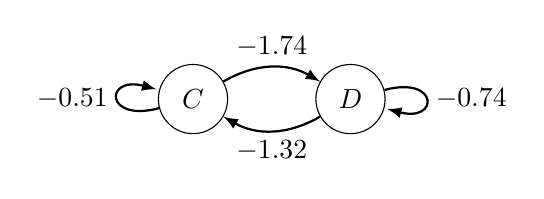
\begin{tikzpicture}[node distance=2cm,->,>=latex,auto,
  every edge/.append style={thick}]
  \node[state] (1) {$C$};
  \node[state] (2) [right of=1] {$D$};  
  \path (1) edge[loop left]  node{$-0.51$} (1)
            edge[bend left]  node{$-1.74$}   (2)
        (2) edge[loop right] node{$-0.74$}  (2)
            edge[bend left] node{$-1.32$}     (1);
\end{tikzpicture}
\end{center}
\begin{table}[h!]
\centering
\begin{tabular}{|l|l|l|}
\hline
\multicolumn{1}{|c|}{$k$} & \multicolumn{1}{c|}{$\ln{P(X_t=k\mid Y_t=C)}$} & $\ln{P(X_t=k \mid Y_t=D)}$ \\ \hline
1                           & -0.69                           & -1.21      \\ \hline
2                           & -0.91                           & -0.69         \\ \hline
3                           & -2.30                           & -1.61      \\ \hline
\end{tabular}
\end{table}

 We observed $X_1 = 1$ and $X_2 = 2$. (Note that taking the maximum of logged probabilities will give you the same result as taking the maximum of probabilities, as log is a monotonically increasing function.)

    
\begin{parts}
    \part[2] Compute $\ln{\omega_1(C)}$ and $\ln{\omega_1(D)}$. If your answers involve decimal numbers, please round your answer to \textbf{TWO} decimal places.
    
    \textit{Note}: Showing your work in these questions is optional, but it is recommended to help us understand where any misconceptions may occur. Only your answer in the left box will be graded.
    
    What is $\ln{\omega_1(C)}$? \\
    \begin{your_solution}[title=$\ln{\omega_1(C)}$,height=2cm,width=3cm]
    % YOUR ANSWER 
    \end{your_solution}
    \begin{your_solution}[title=Work,height=3cm,width=12cm]
    % YOUR ANSWER 
    \end{your_solution}
    
    
    What is $\ln{\omega_1(D)}$? \\
    \begin{your_solution}[title=$\ln{\omega_1(D)}$,height=2cm,width=3cm]
    % YOUR ANSWER 
    \end{your_solution}
    \begin{your_solution}[title=Work,height=3cm,width=12cm]
    % YOUR ANSWER 
    \end{your_solution}
    
    \part[2] (\textbf{Select one}) Which of the following is the most likely sequence of hidden states? 
    
    \begin{list}{}
    % YOUR ANSWER
    % Change \emptycircle to \filledcircle for the appropriate selection/selections
        \item 
            \emptycircle
            % \filledcircle
            $Y_1=C$, $Y_2=C$ 
        \item 
            \emptycircle 
            % \filledcircle
            $Y_1=D$, $Y_2=D$ 
        \item 
            \emptycircle
            % \filledcircle
            $Y_1=D$, $Y_2=C$
        \item 
            \emptycircle
            % \filledcircle
            $Y_1=C$, $Y_2=D$ 
        \item 
            \emptycircle
            % \filledcircle
            Not enough information. 
    \end{list}
    
    
\end{parts}

\clearpage

\sectionquestion{Forward-Backward Algorithm}
\label{hmm-problem}

The following questions should be completed before you start the programming component of this
assignment. To help you prepare to implement the HMM forward-backward algorithm (see Section~\ref{forback} for a detailed explanation), we have provided a small example for you to work through by hand. This toy data set consists of a training set of three sequences with three unique words and two tags, and a validation set with a single sequence composed of the same words occurring in the training set. 

\textbf{Training set:} 
\begin{verbatim}
you     D
eat     C
fish    D

you     D
fish    D
eat     C

eat     C
fish    D
\end{verbatim}

The training word sequences are:
\begin{align*}
    \mathbf{x}^{(1)} &= [\texttt{you eat fish}]^T \\
    \mathbf{x}^{(2)} &= [\texttt{you fish eat}]^T \\
    \mathbf{x}^{(3)} &= [\texttt{eat fish}]^T 
\end{align*}

And the corresponding tags are:
\begin{align*}
    \mathbf{y}^{(1)} &= [D~~C~~D]^T \\
    \mathbf{y}^{(2)} &= [D~~D~~C]^T \\
    \mathbf{y}^{(3)} &= [C~~D]^T
\end{align*}

\textbf{Validation set:}
\begin{verbatim}
fish
eat
you
\end{verbatim}

The validation word sequence is: 
$$
\mathbf{x}_{\text{validation}}= 
\begin{bmatrix}
\texttt{fish eat you}\\
\end{bmatrix}^T
$$

\clearpage
In this question, we define:
\begin{itemize}
    \item Each observed state $x_t \in \{1,2,3\}$, where 1 corresponds to \texttt{you}, 2 corresponds to \texttt{eat}, and 3 corresponds to \texttt{fish}
    \item Each hidden state $Y_t$ $\in \{C,D\}$. Let $s_1 = C$ and $s_2 = D$.
    \item $\mathbf{B}$ is the transition matrix, where $B_{jk} = P(Y_{t} = s_{k} \mid Y_{t-1} = s_{j})$. Here $\mathbf{B}$ is a $2 \times 2$ matrix. 
    \item $\mathbf{A}$ is the emission matrix, where $A_{jk} = P(X_{t} = k \mid Y_{t} = s_{j})$. Here $\mathbf{A}$ is a $2 \times 3$ matrix. As an example, $A_{23}$ denotes $P(X_{t} = 3 \mid Y_{t} = s_{2})$, or the probability that $X_{t}$ corresponds to \texttt{fish} given the hidden state $Y_t = D$.
    \item $\boldsymbol{\pi}$ describes $Y_1$'s initialization probabilities: $\pi_j = P(Y_1 = s_j)$.
    
    For pseudo-code of the Forward-Backward Algorithm, refer to ~\ref{forback}.
    
    
\end{itemize} 
\vspace{0.5cm}

\textit{Note:} Pseudocounts used in section~\ref{learn} should also be used here.

For all numerical answers, round to \textbf{four decimal places} after the decimal point. Showing your work in these questions is optional, but it is recommended to help us understand where any misconceptions may occur. Only your answer in the left box will be graded.

\clearpage
\begin{parts}
    \part[5] Compute $\alpha_2(C)$, the $\alpha$ value associated with the tag ``C'' for the second word in the validation sequence. 
    
    \begin{your_solution}[title=$\alpha_2(C)$,height=2cm,width=3cm]
    % YOUR ANSWER 
    \end{your_solution}
    \begin{your_solution}[title=Work,height=14cm,width=13cm]
    % YOUR ANSWER 
    \end{your_solution}
    
    \part[3] Compute $\beta_2(D)$, the $\beta$ value associated with the tag ``D'' for the second word in the validation sequence. 
    
    \begin{your_solution}[title=$\beta_2(D)$,height=2cm,width=3cm]
    % YOUR ANSWER 
    \end{your_solution}
    \begin{your_solution}[title=Work,height=5.5cm,width=12cm]
    % YOUR ANSWER
    \end{your_solution}    
    
    \clearpage
    \part[3] Predict the tag for the third word in the validation sequence. 
    
    \begin{your_solution}[title=Tag,height=2cm,width=3cm]
    % YOUR ANSWER 
    \end{your_solution}
    \begin{your_solution}[title=Work,height=14cm,width=12cm]
    % YOUR ANSWER 
    \end{your_solution}  
    
    \part[3] Compute the log-likelihood for the entire validation sequence, ``\texttt{fish eat you}".
    
    \begin{your_solution}[title=Log-Likelihood,height=2.5cm,width=3cm]
    % YOUR ANSWER 
    \end{your_solution}
    \begin{your_solution}[title=Work,height=4cm,width=12cm]
    % YOUR ANSWER 
    \end{your_solution} 
    
    \clearpage
    \part[6]Write the following alpha vectors $\alphav_i$ and beta vectors $\betav_i$ in terms of $\Av$, $\Bv$, $\piv$ (indexing them as appropriate), and $\alphav_t$ for any $t$ as well as $\betav_t$ for any $t$. Your solution must rely on matrix-vector operations (e.g. matrix multiplication, elementwise multiplication $\odot$, elementwise addition $\oplus$).
    \begin{subparts}
    \subpart[2]$\alphav_1$\\
    \begin{your_solution}[height=4cm]
    % YOUR ANSWER 
    \end{your_solution} 
    
    \subpart[2]$\alphav_2$\\
    \begin{your_solution}[height=4cm]
        % YOUR ANSWER 
    \end{your_solution} 
    
    \subpart[2]$\betav_2$\\
    \begin{your_solution}[height=4cm]
        % YOUR ANSWER 
    \end{your_solution} 
    \end{subparts}
\end{parts}

\clearpage

\sectionquestion{Empirical Questions}

Return to these questions after implementing your \texttt{learnhmm.py} and \\ \texttt{forwardbackward.py} functions. Please ensure that you have used the log-sum-exp trick in your programming as described in Section \ref{sec:underflow} before answering these empirical questions.

Using the full data set \textbf{en\_data/train.txt} in the handout, use your implementation of\\ \texttt{learnhmm.py} to learn HMM parameters using the first 10, 100, 1000, and 10000 sequences in the file.
Use these learned parameters to perform prediction on both the English \textbf{train.txt} and the \textbf{validation.txt} files with your implementation of \texttt{forwardbackward.py}.
Construct a plot with number of sequences used for training on the x-axis (log-scale with base $e$) and average log likelihood across all sequences from the English \textbf{train.txt} and the \textbf{validation.txt} on the y-axis (see Section~\ref{forback} for details on computing the log data likelihood for a sequence).

Fill in the table with the resulting log likelihood values, rounded to two decimal places, and 
include your plot in the large box.
To receive credit for your plot, you must submit a computer generated plot.
\textbf{DO NOT} hand draw your plot.

\begin{parts}
\part[4] Fill in this table.

% YOUR ANSWER 
% Fill in the table by replacing the ??s with the appropriately calculated likelihood
\begin{table}[h]
    \center
    \begin{tabular}{|m{2cm}|m{3cm}|m{3cm}|}
    \hline
    \# Sequences & Train Average Log-Likelihood & Validation Average Log-Likelihood \\ \hline
    10         &  ?? & ?? \\ \hline
    100        &  ?? & ?? \\ \hline
    1000       &  ?? & ?? \\ \hline
    10000      &  ?? & ?? \\ \hline
    \end{tabular}
    \end{table}

\part[2] Put your plot below:

    \begin{your_solution}[title=Plot,height=10cm,width=15cm]
        % YOUR ANSWER 
        % \begin{center}
        %    \includegraphics[height8.5cm]{allplot.png}
        % \end{center}


    \end{your_solution}



\end{parts}

\clearpage
\newpage
\end{questions}
\newpage
\section{Collaboration Questions}
After you have completed all other components of this assignment, report your answers to these questions regarding the collaboration policy. Details of the policy can be found \href{http://www.cs.cmu.edu/~mgormley/courses/10601/syllabus.html}{here}.
\begin{enumerate}
    \item Did you receive any help whatsoever from anyone in solving this assignment? If so, include full details.
    \item Did you give any help whatsoever to anyone in solving this assignment? If so, include full details.
    \item Did you find or come across code that implements any part of this assignment? If so, include full details.
\end{enumerate}

\begin{your_solution}[height=6cm]
% YOUR ANSWER 

\end{your_solution}

\newpage
\section{Programming (80 points)}
\label{programming}

\subsection{The Task}\label{task}
In the programming section you will implement a named entity recognition system using Hidden Markov Models (HMMs). Named entity recognition (NER) is the task of classifying named entities, typically proper nouns,  into pre-defined categories, such as person, location, or organization. Consider the example sequence below, where each word is appended with a tab and then its tag:

\begin{tabular}{ m{3cm}  m{3cm} } 
    `` & O \\
    Rhinestone & B-ORG \\
    Cowboy & I-ORG \\
    '' & O \\
    ( & O \\
    Larry & B-PER \\
    Weiss & I-PER \\
    ) & O \\ 
    - & O \\
    3:15 & O
\end{tabular}

 \texttt{Rhinestone} and \texttt{Cowboy} are labeled as an organization (\texttt{ORG}), while \texttt{Larry} and \texttt{Weiss} is labeled as a person (\texttt{PER}). Words that aren't named entities are assigned the \texttt{O} tag. The \texttt{B-} prefix indicates that a word is the beginning of an entity, while the \texttt{I-} prefix indicates that the word is inside the entity.

NER is an incredibly important task for a machine to analyze and interpret a body of natural language text. For example, when designing a system that automatically summarizes news articles, it is important to recognize the key subjects in the articles. Another example is designing a trivia bot. If you can quickly extract the named entities from the trivia question, you may be able to more easily query your knowledge base (e.g. type a query into Google) to request information about the answer to the question.

On a technical level, the main task is to implement an algorithm to learn the HMM parameters given the training data and then implement the forward-backward algorithm to perform a smoothing query which we can then use to predict the hidden tags for a sequence of words. 

\subsection{The Dataset}\label{dataset}
\href{https://aclanthology.org/P17-1178.pdf}{WikiANN} is a ``silver standard" dataset that was generated without human labelling. The English Abstract Meaning Representation (AMR) corpus and DBpedia features were used to train an automatic classifier to label Wikipedia articles. These labels were then propagated throughout other Wikipedia articles using the Wikipedia's cross-language links and redirect links. Afterwards, another tagger that self-trains on the existing tagged entities was used to label all other mentions of the same entities, even those with different morphologies (prefixes and suffixes that modify a word in other languages). Finally, the amassed training examples were filtered by ``commonness" and ``topical relatedness" to pick more relevant training data. 

The WikiANN dataset provides labelled entity data for Wikipedia articles in 282 languages. We will be primarily using the English subset, which contains 14,000 training examples and 3,300 test examples, and the French subset, which contains around 7,500 training examples and 300 test examples. 

\clearpage

\subsection{File Formats}\label{formats}
The contents and formatting of each of the files in the handout folder is explained below. 
\begin{enumerate}

\item \textbf{train.txt} This file contains labeled text data that you will use in training your model in the Learning problem (Section \ref{learn}). Specifically, the text contains one word per line that has already been preprocessed, cleaned and tokenized. Every sequence has the following format:

    \texttt{<Word0>\textbackslash t<Tag0>\textbackslash n<Word1>\textbackslash t<Tag1>\textbackslash n ... <WordN>\textbackslash t<TagN>\textbackslash n}

where every \texttt{<WordK>\textbackslash t<TagK>} unit token is separated by a newline. Between each sequence is an empty line. If we have two three-word sequences in our data set, the data will look like so:

    \texttt{<Word0>\textbackslash t<Tag0>\textbackslash n\\<Word1>\textbackslash t<Tag1>\textbackslash n\\<Word2>\textbackslash t<Tag2>\textbackslash n\\\textbackslash n\\}
    \texttt{<Word0>\textbackslash t<Tag0>\textbackslash n\\<Word1>\textbackslash t<Tag1>\textbackslash n\\<Word2>\textbackslash t<Tag2>}
    
\textit{Note:} Word 2 of the second sequence does not end with a newline because it is the end of the data set.

\item \textbf{validation.txt}: This file contains labeled validation data that you will use to evaluate your model. This file has the same format as \textbf{train.txt}.
    
\item \textbf{index\_to\_word.txt, index\_to\_tag.txt}: These files contain a list of all words or tags that appear in the data set. The format is simple:

\begin{tabular}{ m{5cm}  m{5cm} } 
    \textbf{index\_to\_word.txt} & \textbf{index\_to\_tag.txt} \\
    \texttt{<Word0>\textbackslash n} & \texttt{<Tag0>\textbackslash n} \\
    \texttt{<Word1>\textbackslash n} & \texttt{<Tag1>\textbackslash n} \\
    \texttt{<Word2>\textbackslash n} & \texttt{<Tag2>\textbackslash n} \\
    $\vdots$ & $\vdots$
\end{tabular}

In your functions, you will convert the string representation of words or tags to indices corresponding to the location of the word or tag in these files. For example, if \textit{Austria} is on line 729 of \textbf{index\_to\_word.txt}, then all appearances of \textit{Austria} in the data sets should be converted to the index 729. This index will also correspond to locations in the parameter matrices. For example, the word \textit{Austria} corresponds to the parameters in column 729 of the matrix stored in \textbf{hmmemit.txt}. This will be useful for your forward-backward algorithm implementation (see Section~\ref{forback}).

\item \textbf{predicted.txt}: This file contains labeled data that you will use to debug your implementation. The labels in this file are generated by running a reference implementation using the features from \textbf{train.txt}. This file has the same format as \textbf{train.txt}.

\item \textbf{metrics.txt}: This file contains the metrics you will compute for the validation data. The first line should contain the average log likelihood, and the second line should contain the prediction accuracy. There should be a single space after the colon preceding the metric value; see the reference output file for more detail.  

\item \textbf{hmmtrans.txt, hmmemit.txt, hmminit.txt}: These files contain pre-trained model parameters of an HMM that you can use to test your implementation of the Learning and Evaluation and Decoding problems (Sections \ref{learn}, \ref{forback}). The formats of the first two files are the same; each line in these files consists of a conditional probability distribution. In the case of transition probabilities, this distribution corresponds to the probability of transitioning into another state, given a current state. Similarly, in the case of emission probabilities, this distribution corresponds to the probability of emitting a particular symbol, given a current state. Elements in the same row are separated by a space. Each row corresponds to a line of text, using \texttt{\char`\\ n} to create new lines.
    
\textbf{hmmtrans.txt}:

\texttt{<ProbS1S1> <ProbS1S2> ... <ProbS1SN>\textbackslash n}\\
\texttt{<ProbS2S1> <ProbS2S2> ... <ProbS2SN>\textbackslash n}...

\textbf{hmmemit.txt}:

\texttt{<ProbS1Word1> <ProbS1Word2> ... <ProbS1WordN>\textbackslash n}\\
\texttt{<ProbS2Word1> <ProbS2Word2> ... <ProbS2WordN>\textbackslash n}...
     
The format of \textbf{hmminit.txt} is similarly defined except that it only contains a single probability distribution over starting states. Therefore, each row only has a single element.

\textbf{hmminit.txt}:\\
\texttt{<ProbS1>\textbackslash n}\\
\texttt{<ProbS2>\textbackslash n}...

\end{enumerate}

\subsection{Learning}\label{learn}
Your first task is to write a program \texttt{learnhmm.py} to learn the Hidden Markov Model parameters needed to apply the forward-backward algorithm (See Section \ref{forback}). There are three sets of parameters that you will need to estimate: the initialization probabilities {\boldmath$\pi$}, the transition probabilities $\mathbf B$, and the emission probabilities $\mathbf A$. For this assignment, we model each of these probabilities using a multinomial distribution with parameters $ \pi_j=P(Y_1=s_j)$, $ B_{jk} = P(Y_{t}=s_k\mid Y_{t-1}=s_j)$, and $ A_{jk} = P(X_t=k\mid Y_{t}=s_j)$. These can be estimated using maximum likelihood, which results in the following parameter estimates:

\begin{enumerate}
    \item $P(Y_1 = s_j) = \pi_j = \frac{N_{Y_1=s_j}+1}{\sum_{p=1}^{J}(N_{Y_1=s_p}+1)}$, where $N_{Y_1=s_j}$ equals the number of times state $s_j$ is associated with the first word of a sentence in the training data set.
    \item $P(Y_{t} = s_k\mid Y_{t-1}=s_j) = B_{jk}= \frac{N_{Y_t=s_k,Y_{t-1}=s_j}+1}{\sum_{p=1}^J (N_{Y_t=s_p,Y_{t-1}=s_j}+1)}$, where $N_{Y_t=s_k,Y_{t-1}=s_j}$ is the number of times state $s_j$ is followed by state $s_k$ in the training data set.  
    \item $P(X_{t} = k\mid Y_{t}=s_j) = A_{jk}= \frac{N_{X_t=k,Y_t=s_j}+1}{\sum_{p=1}^M (N_{X_t=p,Y_t=s_j}+1)}$, where $N_{X_t=k,Y_t=s_j}$ is the number of times that the state $s_j$ is associated with the word $k$ in the training data set.
\end{enumerate}

Note we add 1 to each count to make a pseudocount. This is slightly different from pure maximum likelihood estimation, but it is useful in improving performance when evaluating unseen cases during evaluation of your validation set.

Your implementation should read in the training data set (\textbf{train.txt}), and then estimate $\bm\pi$, $\mathbf{B}$, and $\mathbf{A}$ using the above maximum likelihood solutions with pseudocounts. 

\clearpage
Your outputs should be in the same format as \textbf{hmminit.txt}, \textbf{hmmtrans.txt}, and \textbf{hmmemit.txt} (including the same number of decimal places to ensure there are no rounding errors during prediction). The autograder runs and evaluates the output from the files generated, using the following command:

\begin{tabbing}
\=\texttt{\$ \textbf{python3} learnhmm.\textbf{py} [args\dots]}\\
\end{tabbing}

Where \texttt{[args\dots]} is a placeholder for six command-line arguments: \texttt{<train\_input>} \texttt{<index\_to\_word>} \texttt{<index\_to\_tag>} \texttt{<hmminit>} \texttt{<hmmemit>} \texttt{<hmmtrans>}. These arguments are described below:
\begin{enumerate}
    \item \texttt{<train\_input>}: path to the training input \texttt{.txt} file (see Section~\ref{dataset})
    \item \texttt{<index\_to\_word>}: path to the \texttt{.txt} file that specifies the dictionary mapping from words to indices. The tags are ordered by index, with the first word having index of 0, the second word having index of 1, etc.
    \item \texttt{<index\_to\_tag>}: path to the \texttt{.txt} file that specifies the dictionary mapping from tags to indices. The tags are ordered by index, with the first tag having index of 0, the second tag having index of 1, etc.
    \item \texttt{<hmminit>}: path to output \texttt{.txt} file to which the estimated initialization probabilities (\boldmath${\pi}$) will be written. The file output to this path should be in the same format as the handout \texttt{hmminit.txt} (see Section~\ref{dataset}).
    \item \texttt{<hmmemit>}: path to output \texttt{.txt} file to which the emission probabilities ($\mathbf A$) will be written. The file output to this path should be in the same format as the handout \texttt{hmmemit.txt} (see Section~\ref{dataset})
    \item \texttt{<hmmtrans>}: path to output \texttt{.txt} file to which the transition probabilities ($\mathbf B$) will be written. The file output to this path should be in the same format as the handout \texttt{hmmtrans.txt} (see Section~\ref{dataset}).
\end{enumerate}
\vspace{0.2 in}
As an example, the following command would run your program on the toy dataset provided in the
handout.
\begin{lstlisting}
$ python3 learnhmm.py toy_data/train.txt toy_data/index_to_word.txt \ 
toy_data/index_to_tag.txt toy_data/hmminit.txt toy_data/hmmemit.txt \ 
toy_data/hmmtrans.txt
\end{lstlisting}

After running the command above, the \texttt{<hmminit>}, \texttt{<hmmemit>}, and \texttt{<hmmtrans>} output files should match the reference files provided in the \texttt{toy\_output} directory.

\newpage

\subsection{Evaluation and Decoding}
\label{forback}

\subsubsection{Forward Backward Algorithm and Minimal Bayes Risk Decoding}

Your next task is to implement the forward-backward algorithm. Suppose we have a set of sequence consisting of $T$ words, $x_1,\dots,x_T$. Each word is associated with a label $Y_t\in\{1,\dots,J\}$. In the forward-backward algorithm we seek to approximate $P(Y_t \mid x_{1:T})$ up to a multiplication constant. This is done by first breaking $P(Y_t \mid x_{1:T})$ into a ``forward'' component and a ``backward'' component as follows:
\begin{align*}
   P(Y_t =s_j \mid x_{1:T}) &\propto P(Y_t=s_j,x_{t+1:T} \mid x_{1:t})\\
   &\propto P(Y_t=s_j \mid x_{1:t})P(x_{t+1:T} \mid Y_t=s_j, x_{1:t})\\
    &\propto P(Y_t=s_j \mid x_{1:t})P(x_{t+1:T} \mid Y_t=s_j)\\ 
     &\propto P(Y_t=s_j, x_{1:t})P(x_{t+1:T} \mid Y_t=s_j) 
\end{align*}



where $P(Y_t=s_j \mid x_1,\dots,x_{t})$ and $P(x_{t+1},\dots,x_T \mid Y_t=s_j)$ are computed by bottom-up dynamic programming approach.

\vspace{0.4 in}
\textbf{Forward Algorithm}



Define $\alpha_t(s_j) = P(Y_t = s_j, x_{1:t})$. This can be rearranged into the following expression (the full derivation can be found in the lecture notes):
\begin{align}
    \label{eqn:alpha}
    \alpha_t(s_j) = A_{jx_t} \sum_{k} B_{kj} \alpha_{t-1}(k)
\end{align}

Using this definition, the $\alpha$'s can be computed using the following dynamic programming procedure:

\begin{lstlisting}[language=Python,escapechar=@]
for t = 1,...,T:
    for j = 1,...,J:
        if t == 1:
            @$\alpha_1(s_j) = \pi_j * A_{j, x_1}$@
        else:
            @$\alpha_t(s_j) = A_{j, x_t} * \sum_k(\alpha_{t-1}(s_k) * B_{k, j})$@
\end{lstlisting}

\vspace{0.2 in}
\textbf{Backward Algorithm}

Define $\beta_t(s_j) = P(x_{t+1:T} \mid Y_t=s_j)$. This can be rearranged into the following expression:
\begin{align}
    \label{eqn:beta}
    \beta_t(s_j) &= \sum_{k=1}^J A_{kx_{t+1}}\beta_{t+1}(s_k)B_{jk}
\end{align}


Just like the $\alpha$'s, the $\beta$'s can also be computed using the following dynamic programming procedure:

\begin{lstlisting}[language=Python,escapechar=@]
for t = T,...,1:
    for j = 1,...,J:
        if t == T:
            @$\beta_T(s_j) = 1$@
        else:
            @$\beta_t(s_j) = \sum_k(A_{k,x_{t+1}}\beta_{t+1}(s_k)B_{j,k})$@
\end{lstlisting}

\clearpage
\textbf{Forward-Backward Algorithm}
As stated above, the goal of the Forward-Backward algorithm is to compute $P(Y_t =s_j \mid x_{1:T})$. This can be done using the following equation:

$$P(Y_t =s_j \mid x_{1:T}) \propto P(Y_t=s_j, x_{1:t})P(x_{t+1:T} \mid Y_t=s_j) $$

After running your forward and backward passes through the sequence, you are now ready to estimate the conditional probabilities as:

$$P(Y_t \mid x_{1:t}) \propto \alpha_t\odot\beta_t$$
where $\odot$ is the element-wise product.

\vspace{0.4 in}
\textbf{Minimum Bayes Risk Prediction}
We will assign tags using the minimum Bayes risk predictor, defined for this problem as follows:

$$\hat{Y}_t = \argmax_{j\in \{1,\dots,J\}} P(Y_t = s_j \mid x_{1:T})$$

To resolve ties, select the tag that appears earlier in the \texttt{<index\_to\_tag>} input file.

\textbf{Computing the Log Likelihood of a Sequence}
When we compute the log likelihood of a sequence, we are interested in the computing the quantity $\log(P(x_{1:T}))$. We can rewrite this in terms of values we have already computed in the forward-backward algorithm as follows:

\begin{align*}
    \log{P(x_{1:T})} &= \log{\big(\sum_j P(x_{1:T},Y_t=s_j)\big)}\\
    &= \log{\big(\sum_j \alpha_T(s_j)\big)}
\end{align*}

\clearpage
\subsubsection{Implementation Details}

You should now write a program \texttt{forwardbackward.py} that implements the forward-backward algorithm. The program will read in validation data and the parameter files produced by \texttt{learnhmm.py}. The autograder runs and evaluates the output from the files generated, using the following command:

\begin{tabbing}
\=\texttt{\$ \textbf{python3} forwardbackward.\textbf{py} [args\dots]}\\
\end{tabbing}

Where \texttt{[args\dots]} is a placeholder for eight command-line arguments:\texttt{<validation\_input>} \texttt{<index\_to\_word>} \texttt{<index\_to\_tag>} \texttt{<hmminit>} \texttt{<hmmemit>} \texttt{<hmmtrans>} \texttt{<predicted\_file>} \texttt{<metric\_file>}. These arguments are described in detail below:
\begin{enumerate}
    \item \texttt{<validation\_input>}: path to the validation input \texttt{.txt} file that will be evaluated by your forward backward algorithm (see Section~\ref{dataset})
    \item \texttt{<index\_to\_word>}: path to the \texttt{.txt} file that specifies the dictionary mapping from words to indices. The tags are ordered by index, with the first word having index of 0, the second word having index of 1, etc. This is the same file as was described for \texttt{learnhmm.py}.
    \item \texttt{<index\_to\_tag>}: path to the \texttt{.txt} file that specifies the dictionary mapping from tags to indices. The tags are ordered by index, with the first tag having index of 0, the second tag having index of 1, etc. This is the same file as was described for \texttt{learnhmm.py}.
    \item \texttt{<hmminit>}: path to input \texttt{.txt} file which contains the estimated initialization probabilities (\boldmath${\pi}$).
    \item \texttt{<hmmemit>}: path to input \texttt{.txt} file which contains the emission probabilities ($\mathbf A$).
    \item \texttt{<hmmtrans>}: path to input \texttt{.txt} file which contains transition probabilities ($\mathbf B$).
    \item \texttt{<predicted\_file>}: path to the output \texttt{.txt} file to which the predicted tags will be written. The file should be in the same format as the \texttt{<validation\_input>} file. 
    \item \texttt{<metric\_file>}: path to the output \texttt{.txt} file to which the metrics will be written. 
\end{enumerate}

As an example, the following command would run your program on the toy dataset provided in the handout.
\begin{lstlisting}
$ python3 forwardbackward.py toy_data/validation.txt \ 
toy_data/index_to_word.txt toy_data/index_to_tag.txt \
toy_data/hmminit.txt toy_data/hmmemit.txt \
toy_data/hmmtrans.txt toy_data/predicted.txt \ 
toy_data/metrics.txt
\end{lstlisting}

After running the command above, the \texttt{<predicted\_file>} output should be:

\begin{lstlisting}
fish    D 
eat     C
you     D

\end{lstlisting}

\clearpage
And the \texttt{<metric\_file>} output should be:

% Change the log likelihood values to reflect last-minute refsol changes
\begin{lstlisting}
Average Log-Likelihood: -3.0438629330222424
Accuracy: 0.3333333333333333
\end{lstlisting}

where average log-likelihood and accuracy are evaluated over the validation set.

Take care that your output has the exact same format as shown above. There should be a single space after the colon preceding the metric value (e.g. a space after \lstinline{Average Log-Likelihood:}). Each line should be terminated by a Unix line ending \lstinline{\n}.

\subsubsection{Log-Space Arithmetic for Avoiding Underflow}
\label{sec:underflow}

Handling underflow properly is a critical step in implementing an HMM. The most generalized way of handling numerical underflow due to products of small positive numbers (like probabilities) is to calculate everything in log-space, i.e., represent every quantity by their logarithm. 

For this homework, using log-space starts with transforming Eq.(\ref{eqn:alpha}) and Eq.(\ref{eqn:beta}) into logarithmic form - you may find the recitation handout helpful. Please use base $e$ (natural log) for logarithm calculation.

After transforming the equations into log form, you may discover calculations of the following type:

$$ \log \sum_i \exp{(v_i)}$$

This may be programmed as is, but $\exp{(v_i)}$ may cause underflow when $v_i$ is large and negative. One way to avoid this is to use the \href{https://www.xarg.org/2016/06/the-log-sum-exp-trick-in-machine-learning/}{log-sum-exp trick}. We provide the pseudocode for this trick in Algorithm \ref{alg:log-sum-exp-trick}:

\begin{algorithm}[H]
    \caption{Log-Sum-Exp Trick}
    \label{alg:log-sum-exp-trick}
    \begin{algorithmic}[1]
        \Procedure{LogSumExpTrick}{($v_1, v_2, \cdots, v_n$)}
            \State $m = \max(v_i)$ for $i=\{1, 2,\cdots, n\}$ 
            \State \textbf{return }{$m + \log(\sum_i\exp(v_i-m))$} 
        \EndProcedure
    \end{algorithmic}
\end{algorithm}

\textbf{Note: The autograder test cases account for numerical underflow using the Log-Sum-Exp Trick. If you do not implement \textbf{forwardbackward.py} with the trick, you might only receive partial credit.}

\subsection{Gradescope Submission}

You should submit your \texttt{learnhmm.py}, \texttt{forwardbackward.py}, and \texttt{utils.py} (if using the functions in the file) to Gradescope. Please do not use other file names. This will cause problems for the autograder to correctly detect and run your code. Please go through the appendix at the end for information on starter-code.

Some additional tips: 
Make sure to read the autograder output carefully. The autograder for Gradescope prints out some additional 
information about the tests that it ran. For this programming assignment we’ve specially designed some buggy implementations that you might implement and will try our best to detect those and give you some more useful feedback in Gradescope’s autograder. Make wise use of autograder’s output for debugging your code.


\textit{Note:} For this assignment, you have 10 submissions to Gradescope before the deadline, but only your last submission will be graded.
\newpage
\section{Appendix}
\subsection{Starter Code}

In this handout, we provide you with some starter code to help you get started, primarily in the form of a \texttt{utils.py} file, along with more skeleton code in the \texttt{learnhmm.py} and \texttt{forwardbackward.py} files. The following functions are provided to you in \texttt{utils.py} to help with file I/O:

\begin{enumerate}
    \item \texttt{make\_dict}: This function takes in a file path and returns a dictionary that maps words or tags to their line numbers (0-indexed).
    
    \item \texttt{parse\_file}: This function takes in a file (train or otherwise), parses it, and returns two lists of lists, one containing sentences and another containing tags.
    
    \item \texttt{write\_predictions}: This function takes in a file path, list of sentences, list of predicted tags, and list of true tags, and writes your computed tags to the given file in the desired format. The function also calculates and returns the accuracy.
    
    \item \texttt{write\_metrics}: This function takes in a file path and relevant metrics, and writes the metrics to the file in the required format.
    
    \item \texttt{get\_matrices}: This function loads your initialization, emission, and transition matrices.
    
\end{enumerate}

For detailed documentation on these functions, please read the function descriptions in the file. You are also encouraged to look at the outputs of these functions to further understand what they're doing.



\end{document}
